\documentclass[../main]{subfiles}

\begin{document}

\clearpage

\setcounter{eqnarray}{0}
\setcounter{equation}{0}
\setcounter{figure}{0}

\part*{第3回}

\subsection{ベクトル場の発散}
3次元空間閉領域Vの表面$\partial$ Vにおけるベクトル場{\bf A}({\bf r})のフラックスの総量$\Phi$ は,1.4節でやった通り,
\begin{equation}
\Phi = \int_{\partial V}^{}{\bf A}\cdot{\bf dS}
\end{equation}
Vの内部から外部へ向かうベクトル場{\bf A}の寄与を一般に正とする.\\
Vの表面$\partial$ Vから発散するフラックスの総量を{\bf 湧き出し}という.\\
閉領域Vの体積を同じくVとすると,Vにおける単位体積あたりの平均の湧き出しは
\begin{equation}
\frac{\Phi}{V}=\frac{1}{V}\int_{\partial V}^{}{\bf A}\cdot {\bf dS}
\end{equation}
閉領域Vをどんどん小さくしていくと,体積Vは0に近づき,閉領域は内部の1点{\bf r}で代表できるようになる.この極限をベクトル場{\bf A}の点{\bf r}における{\bf 発散}(divergence)といい,div{\bf A}({\bf r})と表す.
\begin{itembox}[c]{発散(divergence)}
\begin{equation}
{\rm div}{\bf A}({\bf r})= \lim_{V \to 0}\frac{1}{V}\int_{\partial V}^{}{\bf A}\cdot {\bf dS}
\end{equation}
\end{itembox}

発散は線形性を有する.すなわち点{\bf r}における任意のベクトル場{\bf A},{\bf B}について,c	を定数として以下が成り立つ.
\begin{equation}
{\rm div}({\bf A}+{\bf B})={\rm div}{\bf A}+{\rm div}{\bf B}
\end{equation}
\begin{equation}
{\rm div}(c{\bf A})=c\,{\rm div}{\bf A}
\end{equation}
${\bf A}({\bf r})={\bf A}(x,y,z)=(A_x(x,y,z),A_y(x,y,z),A_z(x,y,z))$と表すとき,以下の式が成り立つ.\footnote{ここでは扱わなかったが,微分演算子$\nabla:=\left( \frac{\partial}{\partial x} \, \frac{\partial}{\partial y} \, \frac{\partial}{\partial z} \right) $を用いると, ${\rm div}{\bf A}=\nabla \cdot {\bf A}$と表記が簡単になる.}
\begin{itembox}[c]{}
\begin{equation}
{\rm div}{\bf A}=\frac{\partial A_x}{\partial x}+\frac{\partial A_y}{\partial y}+\frac{\partial A_z}{\partial z}
\end{equation}
\end{itembox}

\newpage
{\bf 証明}\\

\begin{figure}[htbp]
 \begin{center}
  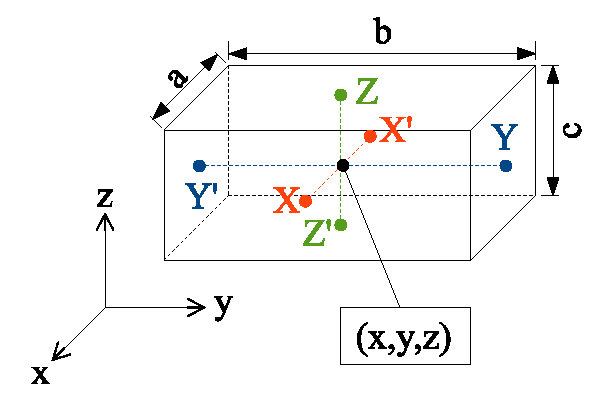
\includegraphics[width=80mm]{3.1.eps}
 \end{center}
 \caption{}
 \label{fig:one}
\end{figure}
点${\bf r}=(x,y,z)$を中心とする閉領域Vを考える.\\
発散を考えるとき$V \to 0$の極限を考えるので,Vは勝手な形にしても問題ない,ここでは全ての面がxy,yz,zx平面のいずれかに平行な直方体とする.\\
微小な直方体であるから,6面それぞれのフラックスは,それぞれの面の中心の点におけるベクトル場の面に垂直な成分と面積の積となる.\\
各面に図1のように記号をふる.
各面のフラックスは,Vの内部から外部に向かう{\bf A}の寄与を正とする事と,座標軸の取り方に注意すると,
\begin{equation}
\left \{
\begin{array}{l}
X\,: A_x(x+\frac{a}{2},y,z)bc\\
X': -A_x(x-\frac{a}{2},y,z)bc\\
Y\,: A_y(x,y+\frac{b}{2},z)ac\\
Y': -A_y(x,y-\frac{b}{2},z)ac\\
Z\,: A_z(x,y,z+\frac{c}{2})ab\\
Z': -A_z(x,y,z-\frac{c}{2})ab
\end{array}
\right.
\end{equation}
したがって点${\bf r}=(x,y,z)$における発散は,Vを微小にしていき,
\begin{eqnarray}
\frac{1}{V}\int_{\partial V}^{}{\bf A}\cdot {\bf dS} \to \frac{1}{abc} &\{A_x(x+\frac{a}{2},y,z)bc & -A_x(x-\frac{a}{2},y,z)bc \\
 &+A_y(x,y+\frac{b}{2},z)ac&-A_y(x,y-\frac{b}{2},z)ac \\
&+A_z(x,y,z+\frac{c}{2})ab&-A_z(x,y,z-\frac{c}{2})ab \}
\end{eqnarray}
はじめの2項だけに着目する.(y,zは変化しないので$A_x(x+\frac{a}{2})bc-A_x(x-\frac{a}{2})bc$として,xの関数とみる.)\\
$A_x(x+\frac{a}{2}),A_x(x-\frac{a}{2})$ のxまわりのTaylor展開は,\\
\begin{equation}
A_x(x+\frac{a}{2})=A_x(x)+\frac{\partial A_x}{\partial x}(x+\frac{a}{2}-x)+\frac{1}{2}\frac{\partial^2 A_x}{\partial x^2}(x+\frac{a}{2}-x)^2+...
\end{equation}
\begin{equation}
A_x(x-\frac{a}{2})=A_x(x)+\frac{\partial A_x}{\partial x}(x-\frac{a}{2}-x)+\frac{1}{2}\frac{\partial^2 A_x}{\partial x^2}(x-\frac{a}{2}-x)^2+...
\end{equation}
それぞれの式の第3項以降には,いま$a \to 0$で考えているため,「微小量の2乗以上」が現れる.これを無視すると,(一次近似)
\begin{eqnarray}
A_x(x+\frac{a}{2})=A_x(x)+\frac{a}{2}\frac{\partial A_x}{\partial x}\\
A_x(x-\frac{a}{2})=A_x(x)-\frac{a}{2}\frac{\partial A_x}{\partial x}
\end{eqnarray}
差をとると,
\begin{eqnarray}
&bc&\{A_x(x+\frac{a}{2})-A_x(x-\frac{a}{2})\}\\
&=&bc\{ A_x(x)+\frac{a}{2}\frac{\partial A_x}{\partial x}-A_x(x)+\frac{a}{2}\frac{\partial A_x}{\partial x} \} \\
&=&abc\frac{\partial A_x}{\partial x}
\end{eqnarray}
$A_y,A_z$の項についても同様に考えると, $ abc\frac{\partial A_y}{\partial y},abc\frac{\partial A_z}{\partial z} $となる.したがって,
\begin{eqnarray}
\frac{1}{V}\int_{\partial V}^{}{\bf A}\cdot {\bf dS} \to &\frac{1}{abc}&\left(abc\frac{\partial A_x}{\partial x}+abc\frac{\partial A_y}{\partial y}+abc\frac{\partial A_z}{\partial z} \right)\\
&=&\frac{\partial A_x}{\partial x}+\frac{\partial A_y}{\partial y}+\frac{\partial A_z}{\partial z}
\end{eqnarray}
\begin{flushright}
(証明終)
\end{flushright}

\subsection{体積積分}
$\varphi=\varphi({\bf r})$をスカラー場とする.\\
領域Vに対し,スカラー場$\varphi$の体積積分を定義したい.\\
Vを微小領域$V_1,V_2,...$に分割していき,それぞれの領域を代表するスカラー場の値を領域内の点${\bf r}_i$での値とする.スカラー場$\varphi({\bf r}_i)$と微小領域$V_i$の積を領域Vにわたって足し合わせ,$V_i \to 0$とする.この極限をスカラー場$\varphi$の体積積分と定義する.
\begin{itembox}[c]{体積積分}
\begin{equation}
\int_{V}^{}\varphi({\bf r})dV = \lim_{V_i \to 0}\sum_{i}^{}\varphi({\bf r}_i)V_i
\end{equation}
\end{itembox}

{\bf 例}\\
V内で$\varphi=c$(一定)のとき,
\begin{equation}
\int_{V}^{}\varphi dV = \lim_{V_i \to 0}\sum_{i}^{}c V_i = cV
\end{equation}

\subsection{Gaussの定理と,Gaussの法則の微分形}
\begin{itembox}[c]{Gaussの定理}
\begin{equation}
\int_{\partial V}^{}{\bf A}\cdot {\bf dS} = \int_{V}^{}{\rm div}{\bf A}dV
\end{equation}
\begin{equation}
\mbox{面積分 \,\,\,\,\,\,\, 体積積分}
\end{equation}
\end{itembox}


\newpage
{\bf 証明}\\
\begin{figure}[htbp]
 \begin{center}
  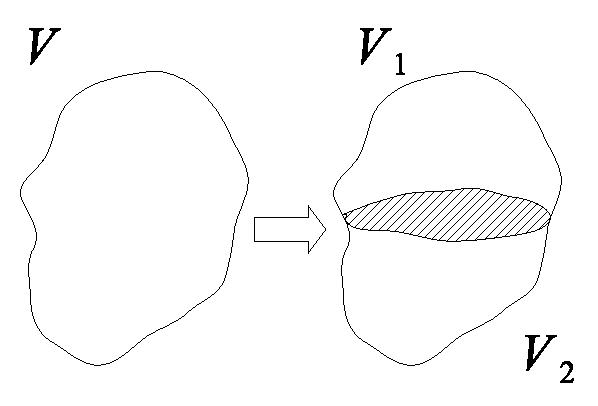
\includegraphics[width=60mm]{3.2.eps}
 \end{center}
 \caption{}
 \label{fig:one}
\end{figure}
任意の閉領域Vを$V_1$と$V_2$に分割するとき,新たに生じた面を通過するベクトル場は,$V_1$と$V_2$に対して,大きさは同じだが,方向が\\
$V_1$にとって内 $\to$ 外のとき, $V_2$にとって,外 $\to$ 内\\
$V_1$にとって外 $\to$ 内のとき, $V_2$にとって,内 $\to$ 外\\
となり,方向が逆となるから,新たに生じる面からの,フラックスへの寄与は0となる.したがって,\\
\begin{equation}
\int_{\partial V}^{}{\bf A}\cdot {\bf dS} = \int_{\partial V_1}^{}{\bf A}\cdot {\bf dS} + \int_{\partial V_2}^{}{\bf A}\cdot {\bf dS}
\end{equation}
分割を繰り返すと,
\begin{equation}
\int_{\partial V}^{}{\bf A}\cdot {\bf dS} = \sum_{i}^{} \int_{\partial V_i}^{}{\bf A}\cdot {\bf dS}=\sum_{i}^{} V_i \frac{1}{V_i} \int_{\partial V_i}^{}{\bf A}\cdot {\bf dS}
\end{equation}
$V_i$を微小とすると次々と
\begin{eqnarray}
\int_{\partial V}^{}{\bf A}\cdot {\bf dS} &=&\sum_{i}^{} V_i \frac{1}{V_i} \int_{\partial V_i}^{}{\bf A}\cdot {\bf dS}\\
&\to& \sum_{i}^{} V_i {\rm div}{\bf A}({\bf r_i})\\
&\to& \int_{V}^{}{\rm div}{\bf A}dV
\end{eqnarray}
\begin{flushright}
(証明終)
\end{flushright}

\begin{itembox}[c]{Gaussの法則}
\begin{equation}
\varepsilon_0 \int_{\partial V}^{}{\bf E}\cdot {\bf dS}=({\mbox V内の全電荷})=\int_{V}^{}\rho({\bf r})dV \, [C]
\end{equation}
\end{itembox}
$\rho({\bf r})$: {\bf 電荷密度}(スカラー場)[$Cm^{-3}$]\\

Gaussの定理から,
\begin{eqnarray}
\varepsilon_0 \int_{\partial V}^{}{\bf E}\cdot {\bf dS} = \varepsilon_0 \int_{V}^{}{\rm div}{\bf E}dV = \int_{V}^{}\rho({\bf r})dV \\
\int_{V}^{} ( \varepsilon_0{\rm div}{\bf E}dV - \rho ) dV =0
\end{eqnarray}
領域Vは任意であるから,
\begin{eqnarray}
\varepsilon_0{\rm div}{\bf E}\,dV - \rho =0
\end{eqnarray}

\begin{itembox}[c]{Gaussの法則の微分形}
\begin{eqnarray}
{\rm div}{\bf E}=\frac{\rho}{\varepsilon_0}
\end{eqnarray}
\end{itembox}
これはMaxwell方程式のひとつでもある.


{\bf 例\, 半径aの球一様に分布した電荷}\\
1.6節でやったように,\\
\begin{equation}
{\bf E}=
\left \{
\begin{array}{l}
\frac{Q}{4 \pi \varepsilon_0}\frac{{\bf r}}{r^3} \, (r > a)\\
\\
\frac{Q}{4 \pi \varepsilon_0 a^3}{\bf r} \, (r \leq a)
\end{array}
\right.
\end{equation}
\begin{equation}
(r=|{\bf r}|=\sqrt[]{\mathstrut x^2+y^2+z^2})
\end{equation}
$r > a$のとき\\
\begin{eqnarray}
{\rm div}{\bf E}&=&\frac{Q}{4 \pi \varepsilon_0} \left\{\frac{\partial}{\partial x}\left(\frac{x}{r^3}\right)+\frac{\partial}{\partial y}\left(\frac{y}{r^3}\right)+\frac{\partial}{\partial z}\left(\frac{z}{r^3}\right) \right\} \\
&=&\frac{Q}{4 \pi \varepsilon_0} \left( \frac{1}{r^3}-3 \cdot \frac{x}{r^4} \cdot \frac{2x}{2r}+\frac{1}{r^3}-3 \cdot \frac{y}{r^4} \cdot \frac{2y}{2r}+\frac{1}{r^3}-3 \cdot \frac{z}{r^4} \cdot \frac{2z}{2r} \right) \\
&=&\frac{Q}{4 \pi \varepsilon_0} \left( \frac{1}{r^3}-\frac{3x^2}{r^5}+\frac{1}{r^3}-\frac{3y^2}{r^5}+\frac{1}{r^3}-\frac{3z^2}{r^5} \right) \\
&=&\frac{Q}{4 \pi \varepsilon_0} \left( \frac{3}{r^3}-\frac{3r^2}{r^5} \right) = 0
\end{eqnarray}
$r \leq a$のとき\\
\begin{eqnarray}
{\rm div}{\bf E}&=&\frac{Q}{4 \pi \varepsilon_0 a^3} \left( \frac{\partial x}{\partial x}+\frac{\partial y}{\partial y}+\frac{\partial z}{\partial z} \right)\\
&=&\frac{3Q}{4 \pi \varepsilon_0 a^3}=\frac{1}{\varepsilon_0}\frac{Q}{\left( \frac{4 \pi a^3}{3} \right)}=\frac{\rho}{\varepsilon_0}
\end{eqnarray}

\end{document}
